\section{Neurophenomenology of KT}




%%%%%%%%%%%%%%%%%%%%%%%%%%%%%%%%%%%%%%%%%%%%%%%%%%%%%%%%%%%%%%%%%%%
\begin{frame}[label=ladila]{Altered states of \SEP}
  
 Neurophenomenology defines a methodological strategy for integrating phenomenological and neurobiological accounts: 1P  (phenomenology---subjective) and 3P (physiology, behavior---objective) data \citep{Varela:1996aa}. \vfill
 
 Altered states of consciousness such as psychedelics or meditation offer an interesting context to study the effect of perturbing the mechanisms of \SEP.\vfill
 
Meditative states are associated with the global dissolution of the embodied self  \citep{Millire2018} and can  serve as unique models for  investigation of self-dissolution (disengagement of self-models).\vfill
 
 As an  objective measure of structured experience, we can analyze descriptive narratives in speech form through state-of-the-art computational analysis (NLP) to establish  metrics on text structure such as semantic coherence and speech disorganization index~\citep{Sanz:2021, Tagliazucchi:2022, Mota:2017}.
 
 
\end{frame}

 
  %%%%%%%%%%%%%%%%%%%%%%%%%%%%%%%%%%%%%%%%%%%%%%%%%%%%%%
  \begin{frame}{The dimensions of structured experience}
  \begin{columns}
\begin{column}{0.5\textwidth}
    
  The structure of the reduced manifold represents the structure of experience, while model accuracy and breath ($\mathcal M$) map into the realism and breath of experience.
\vspace{1cm}
  
  This is the map of the three dimensions of \SEP  into mathematical concepts. 
 
\end{column}
\begin{column}{0.5\textwidth}  
    \begin{center}
         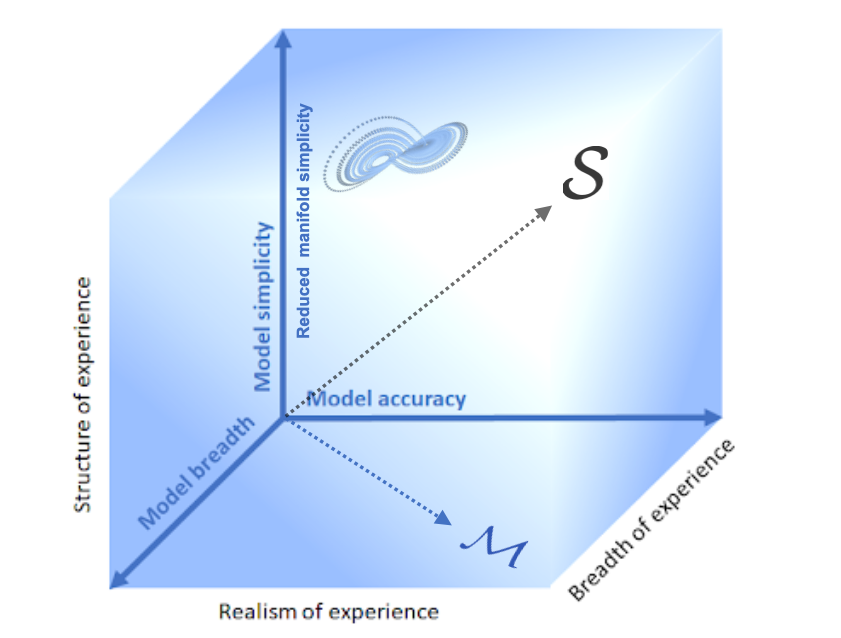
\includegraphics[height=6cm]{img/3dKT2.png}
     \end{center}
\end{column}
\end{columns}

\end{frame}
